
\section{Common Vulnerability Scoring System (CVSS)}

There are various ways to score or calculate severity ratings of
vulnerabilities. The Common Vulnerability Scoring System (CVSS) is an industry
standard for performing these calculations. Many scanning tools will apply
these scores to each finding as a part of the scan results, but it's important
that we understand how these scores are derived in case we ever need to
calculate one by hand or justify the score applied to a given vulnerability.
Risk Scoring

The CVSS system helps categorize the risk associated with an issue and allows
organizations to prioritize issues based on the rating. The CVSS scoring
consists of the exploitability and impact of an issue. The exploitability
measurements consist of access vector, access complexity, and authentication.
The impact metrics consist of the CIA triad, including confidentiality,
integrity, and availability.

\begin{figure}
  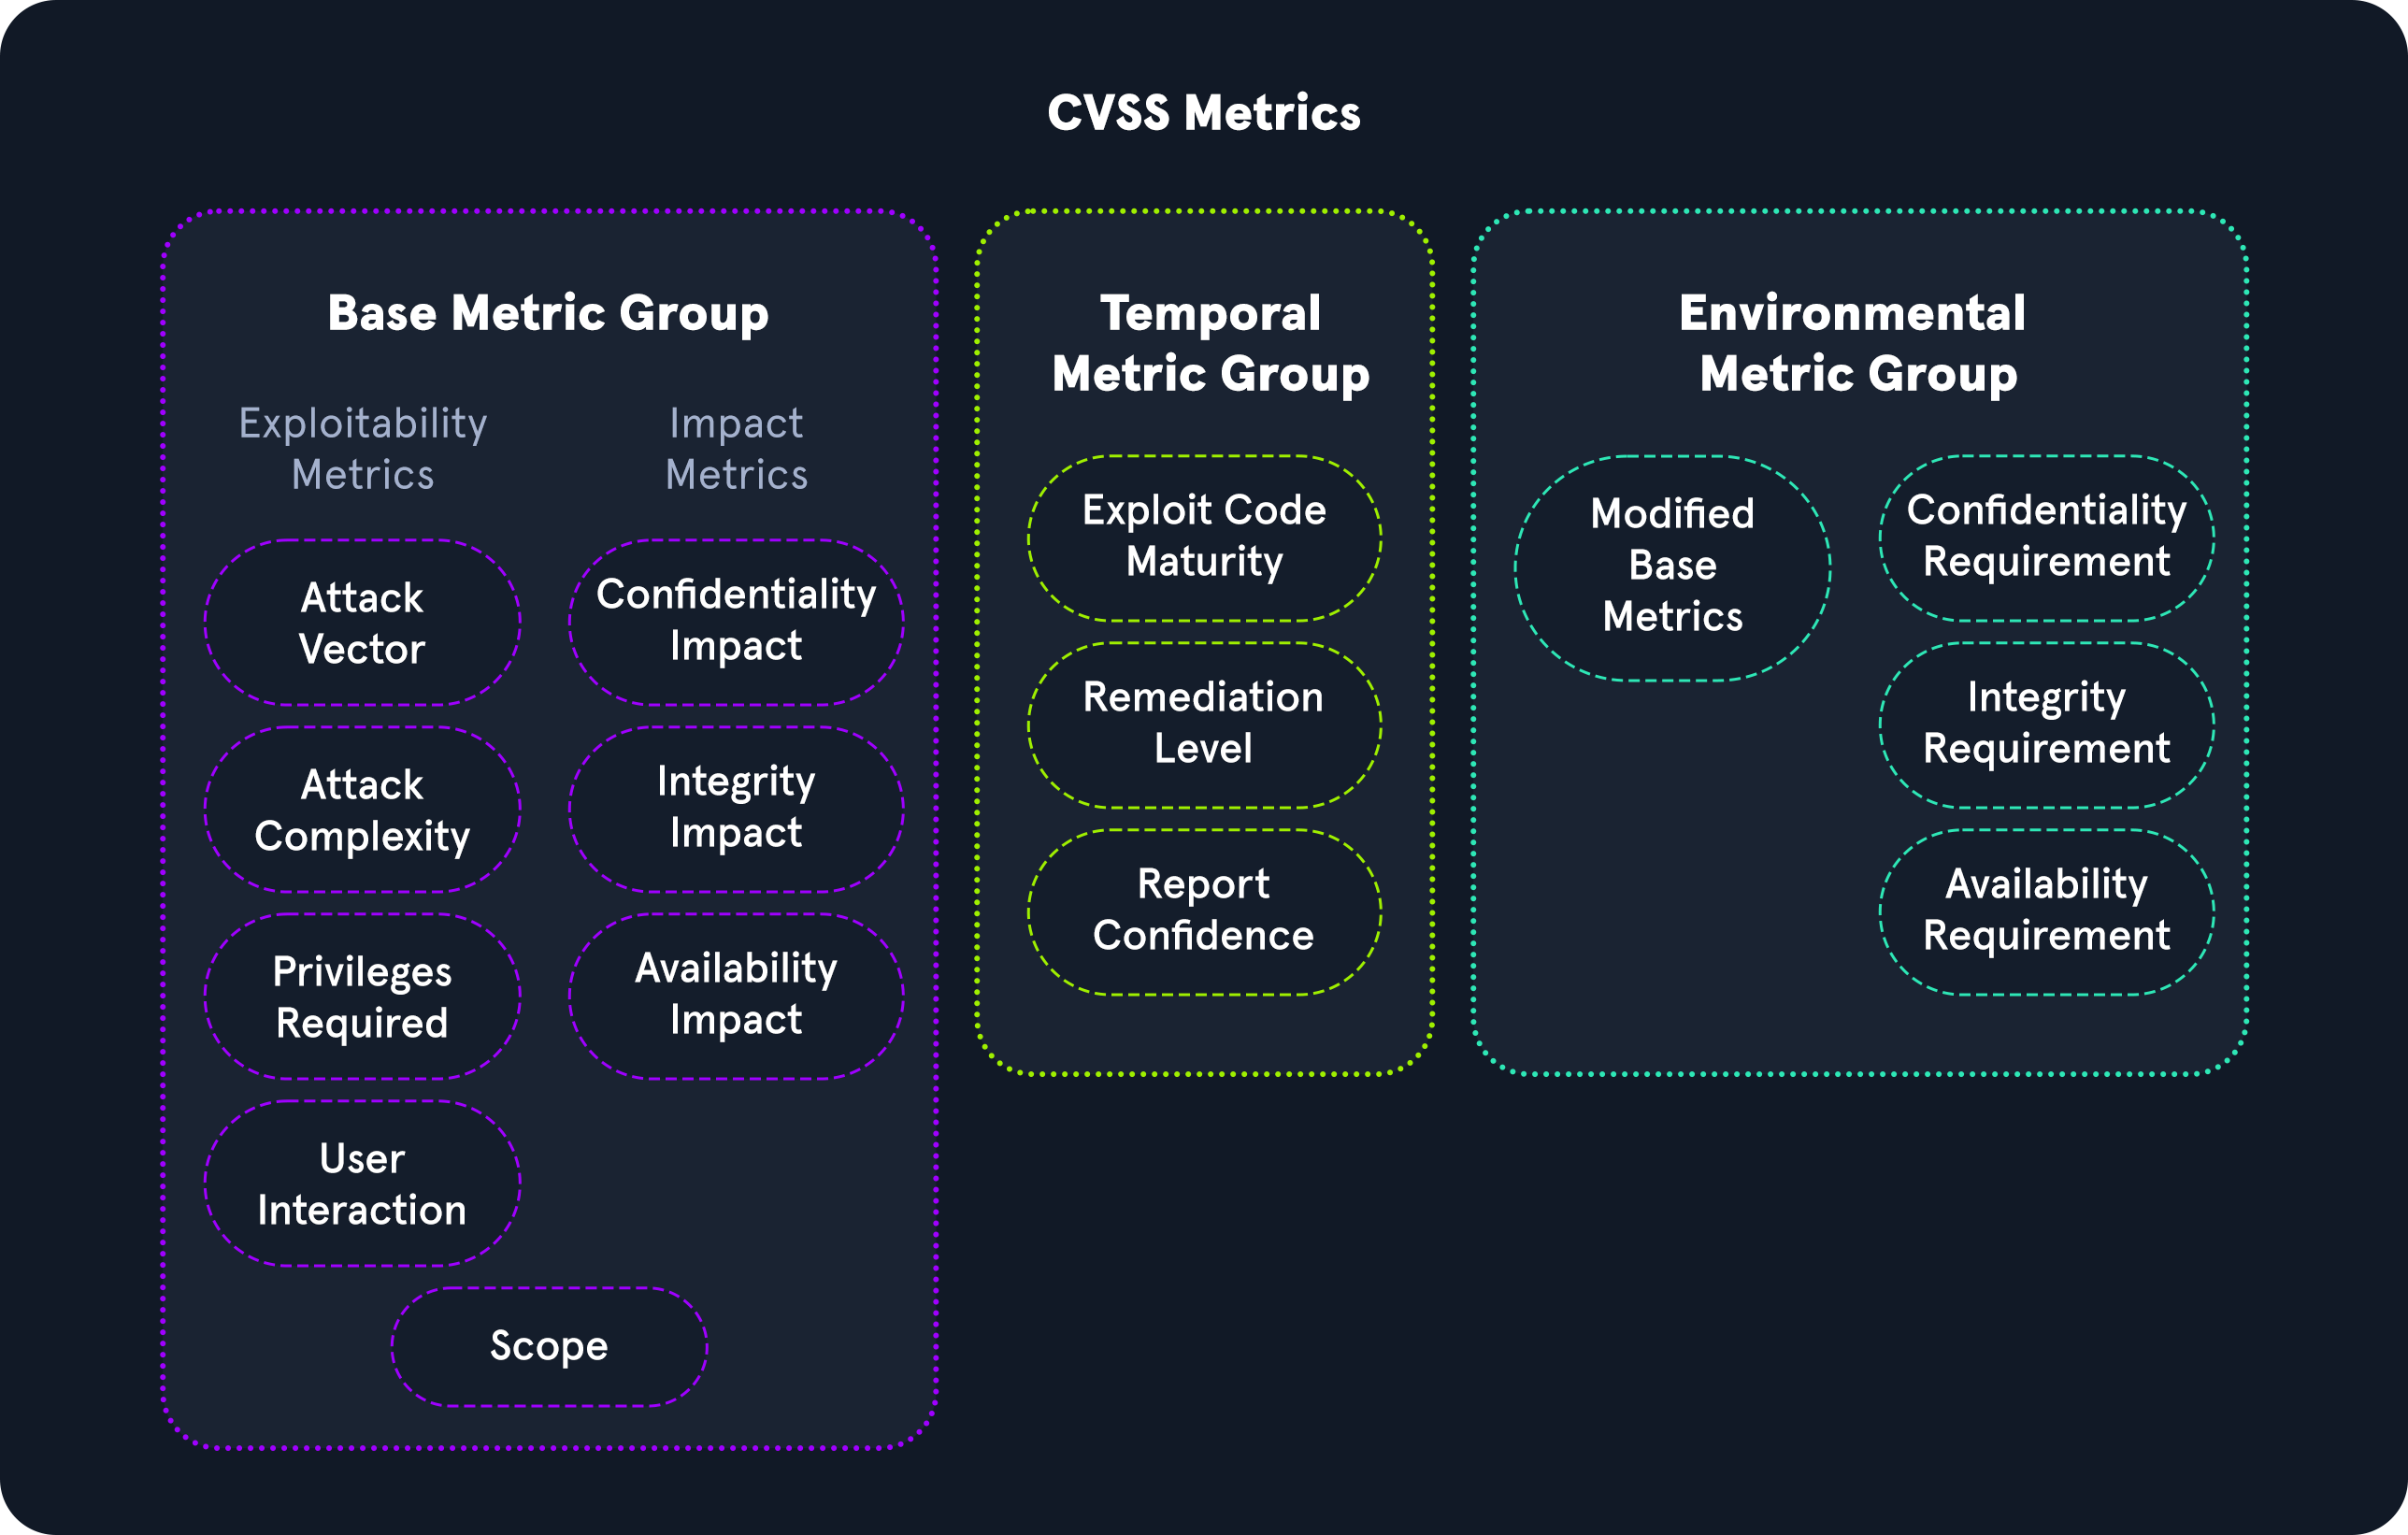
\includegraphics[width=\linewidth]{intro/vuln/images/cvss.png}
  \caption{CVSS}
  \label{fig:pentest-vul-cvss}
\end{figure}
\subsection{Base Metric Group}

The CVSS base metric group represents the vulnerability characteristics and consists of exploitability metrics and impact metrics.

\subsubsection{Exploitability Metrics}

The Exploitability metrics are a way to evaluate the technical means needed to exploit the issue using the metrics below:
\begin{itemize}
    \item Attack Vector
    \item Attack Complexity
    \item Privileges Required
    \item User Interaction
\end{itemize}

\subsubsection{Impact Metrics}

The Impact metrics represent the repercussions of successfully exploiting an issue and what is impacted in an environment, and it is based on the CIA triad. The CIA triad is an acronym for Confidentiality, Integrity, and Availability.

\subsection{Temporal Metric Group}

The Temporal Metric Group details the availability of exploits or patches regarding the issue.

\subsubsection{Exploit Code Maturity}

The Exploit Code Maturity metric represents the probability of an issue being exploited based on ease of exploitation techniques. There are various metric values associated with this metric, including Not Defined, High, Functional, Proof-of-Concept, and Unproven.

A 'Not Defined' value relates to skipping this particular metric. A 'High' value represents an exploit consistently working for the issue and is easily identifiable with automated tools. A Functional value indicates there is exploit code available to the public. A Proof-of-Concept demonstrates that a PoC exploit code is available but would require changes for an attacker to exploit the issue successfully.

\subsubsection{Remediation Level}

The Remediation level is used to identify the prioritization of a vulnerability. The metric values associated with this metric include Not Defined, Unavailable, Workaround, Temporary Fix, and Official Fix.

A 'Not Defined' value relates to skipping this particular metric. An 'Unavailable' value indicates there is no patch available for the vulnerability. A 'Workaround' value indicates an unofficial solution released until an official patch by the vendor. A 'Temporary Fix' means an official vendor has provided a temporary solution but has not released a patch yet for the issue. An 'Official Fix' indicates a vendor has released an official patch for the issue for the public.

\subsubsection{Report Confidence}

Report Confidence represents the validation of the vulnerability and how accurate the technical details of the issue are. The metric values associated with this metric include Not Defined, Confirmed, Reasonable, and Unknown.

A 'Not Defined' value relates to skipping this particular metric. A 'Confirmed' value indicates there are various sources with detailed information confirming the vulnerability. A 'Reasonable' value indicates sources have published information about the vulnerability. However, there is no complete confidence that someone would achieve the same result due to missing details of reproducing the exploit for the issue.

\subsection{Environmental Metric Group}

The Environmental metric group represents the significance of the vulnerability of an organization, taking into account the CIA triad.

\subsubsection{Modified Base Metrics}

The Modified Base metrics represent the metrics that can be altered if the affected organization deems a more significant risk in Confidentiality, Integrity, and Availability to their organization. The values associated with this metric are Not Defined, High, Medium, and Low.

A 'Not Defined' value would indicate skipping this metric. A 'High' value would mean one of the elements of the CIA triad would have astronomical effects on the overall organization and customers. A 'Medium' value would indicate one of the elements of the CIA triad would have significant effects on the overall organization and customers. A 'Low' value would mean one of the elements of the CIA triad would have minimal effects on the overall organization and customers.

\subsection{Calculating CVSS Severity}

The calculation of a CVSS v3.1 score takes into account all the metrics
discussed in this section. The National Vulnerability Database has a calculator
available to the public
\href{https://nvd.nist.gov/vuln-metrics/cvss/v3-calculator}{here}.
